\section{Experiment 2}
\subsection{Methodology} \label{method-2}
The second experiment extends upon the first one, and focus in an HCI setting.
In other words, does the same result from the experiment one apply to another domain?
Different from political and public-opinion surveys, HCI surveys related to preference elicitation often focus on preferences design and experiences.
This issue made measuring participant's real preference much more non-trivial to measure compared to the donation task.
Thus, we developed a buyback mechanism and observed participants' behaviors in that task.
This experiment also acts as a concrete example of how QV can be incorporated in HCI.

\subsection{Choice of HCI Research Question}
To prevent from coming up with an entire new HCI study that requires sophisticated verification.
We want a well-explored HCI topic that we could rely on to ensure ecological validity.
Most HCI research uses Likert scale surveys to understand participant's opinions across one or more devices, designs, or interfaces.
%One could view this as one form of eliciting one out of $K$. 
However, reproducing one of these experiences can be costly and difficult because of the availability of these devices, designs, or interfaces.
Therefore, we turn to the other type of use case, where UX/UI researchers aimed to prioritize features and elements that their customers care about.
We see these forms often as online feedback forms.

Research on video and audio elements of video playback from the lens of HCI has been relatively mature.
Contributions has been made to fields like multi-media conferencing \cite{watson1996evaluating}, video-audio perception \cite{chen2006cognitive, molnar2015assessing}and more specifically trade-offs between video and audio elements under network monetary constraints \cite{molnar2013comedy, oeldorf2012bad}.
\textcite{oeldorf2012bad} conducted a study to understand how users with bandwidth constraints made trade-offs covering the broadest range of elements to the best of our knowledge, across multiple video and audio elements. 
They examined participants' attitudes between three video bit rates, three video frame rates, and two audio sampling rates across three types of video content.
Participants were asked to rate the overall quality, video quality, audio quality, and enjoyment level on a 5-point Likert scale in each condition. 
The conclusion was drawn using the mean and standard deviation of the survey results.
%This is a typical study where the goal is to find one or some of the $K$ elements to choose from when under constraint.
Thus, we follow a similar scenario: 
If there is limited bandwidth, what are the participant's attitudes across a broader range of video and audio elements?
We like to compare how Likert scaled survey and QV reflects people's underlying preferences. 
Based on related works, we selected five video elements to alter in our experiments. 
These elements includes: (1) Stability of Video Imagery \cite{claypool1999effects}, (2) Stability of Audio \cite{claypool1999effects}, (3) Quality of audio \cite{oeldorf2012bad, noll1993wideband}, (4) Quality of the video \cite{oeldorf2012bad, knoche2008low}, and (5) Audio-Video Synchronization \cite{steinmetz1996human}. 
The ``Stability of Video Imagery'' refers to how the screen would freeze with the previous frame. 
This element changes when video packets are lost during transmission. 
We construct four levels of packet loss in our experiment: 20\%, 8\%, 4\%, and 0\% of the data lost. 
The ``Stability of Audio'' refers to the audio of the video dropping occasionally during playback. 
Again, this happens when there are lost audio packets during transmission. 
In our experiment, we constructed four levels of stability with 20\%, 8\%, 4\%, and 0\% of audio pack loss. 
The ``Quality of audio'' refers to how clear or muffled are the sound quality. 
The difference in audio quality occurs because of the different audio sampling rate, which impacts the size of the file. 
In the experiment, we use 8kHz, 11kHz, 16kHz, and 48kHz encoded audio files. 
The ``Quality of the video'' refers to how sharp the visuals in the video are.
The quality of the video is alternated by changing the video resolution and fitted into the same display, which we used 210x280, 294x392, 364x486, and 420x560 in our experiment to demonstrate changes in the pixel density per inch.
Finally, the ``Video-audio Synchronization'' is how well are the video visuals synchronized with the audio playback.
In our experiment, we have the audio play 1850, 1615, 1050, or 0 milliseconds ahead of the video.
% Details of these elements are discussed in the next subsection.

% \begin{figure}[htpb]
%     \centering
%     \includegraphics[width=\textwidth, keepaspectratio=true]{resources/exp_2_video.png}
%     \caption{
%         Real-time Video Element Interface
%     }
%     \label{fig:exp_2_video}
% \end{figure}

\begin{figure}[htpb]
    \centering
    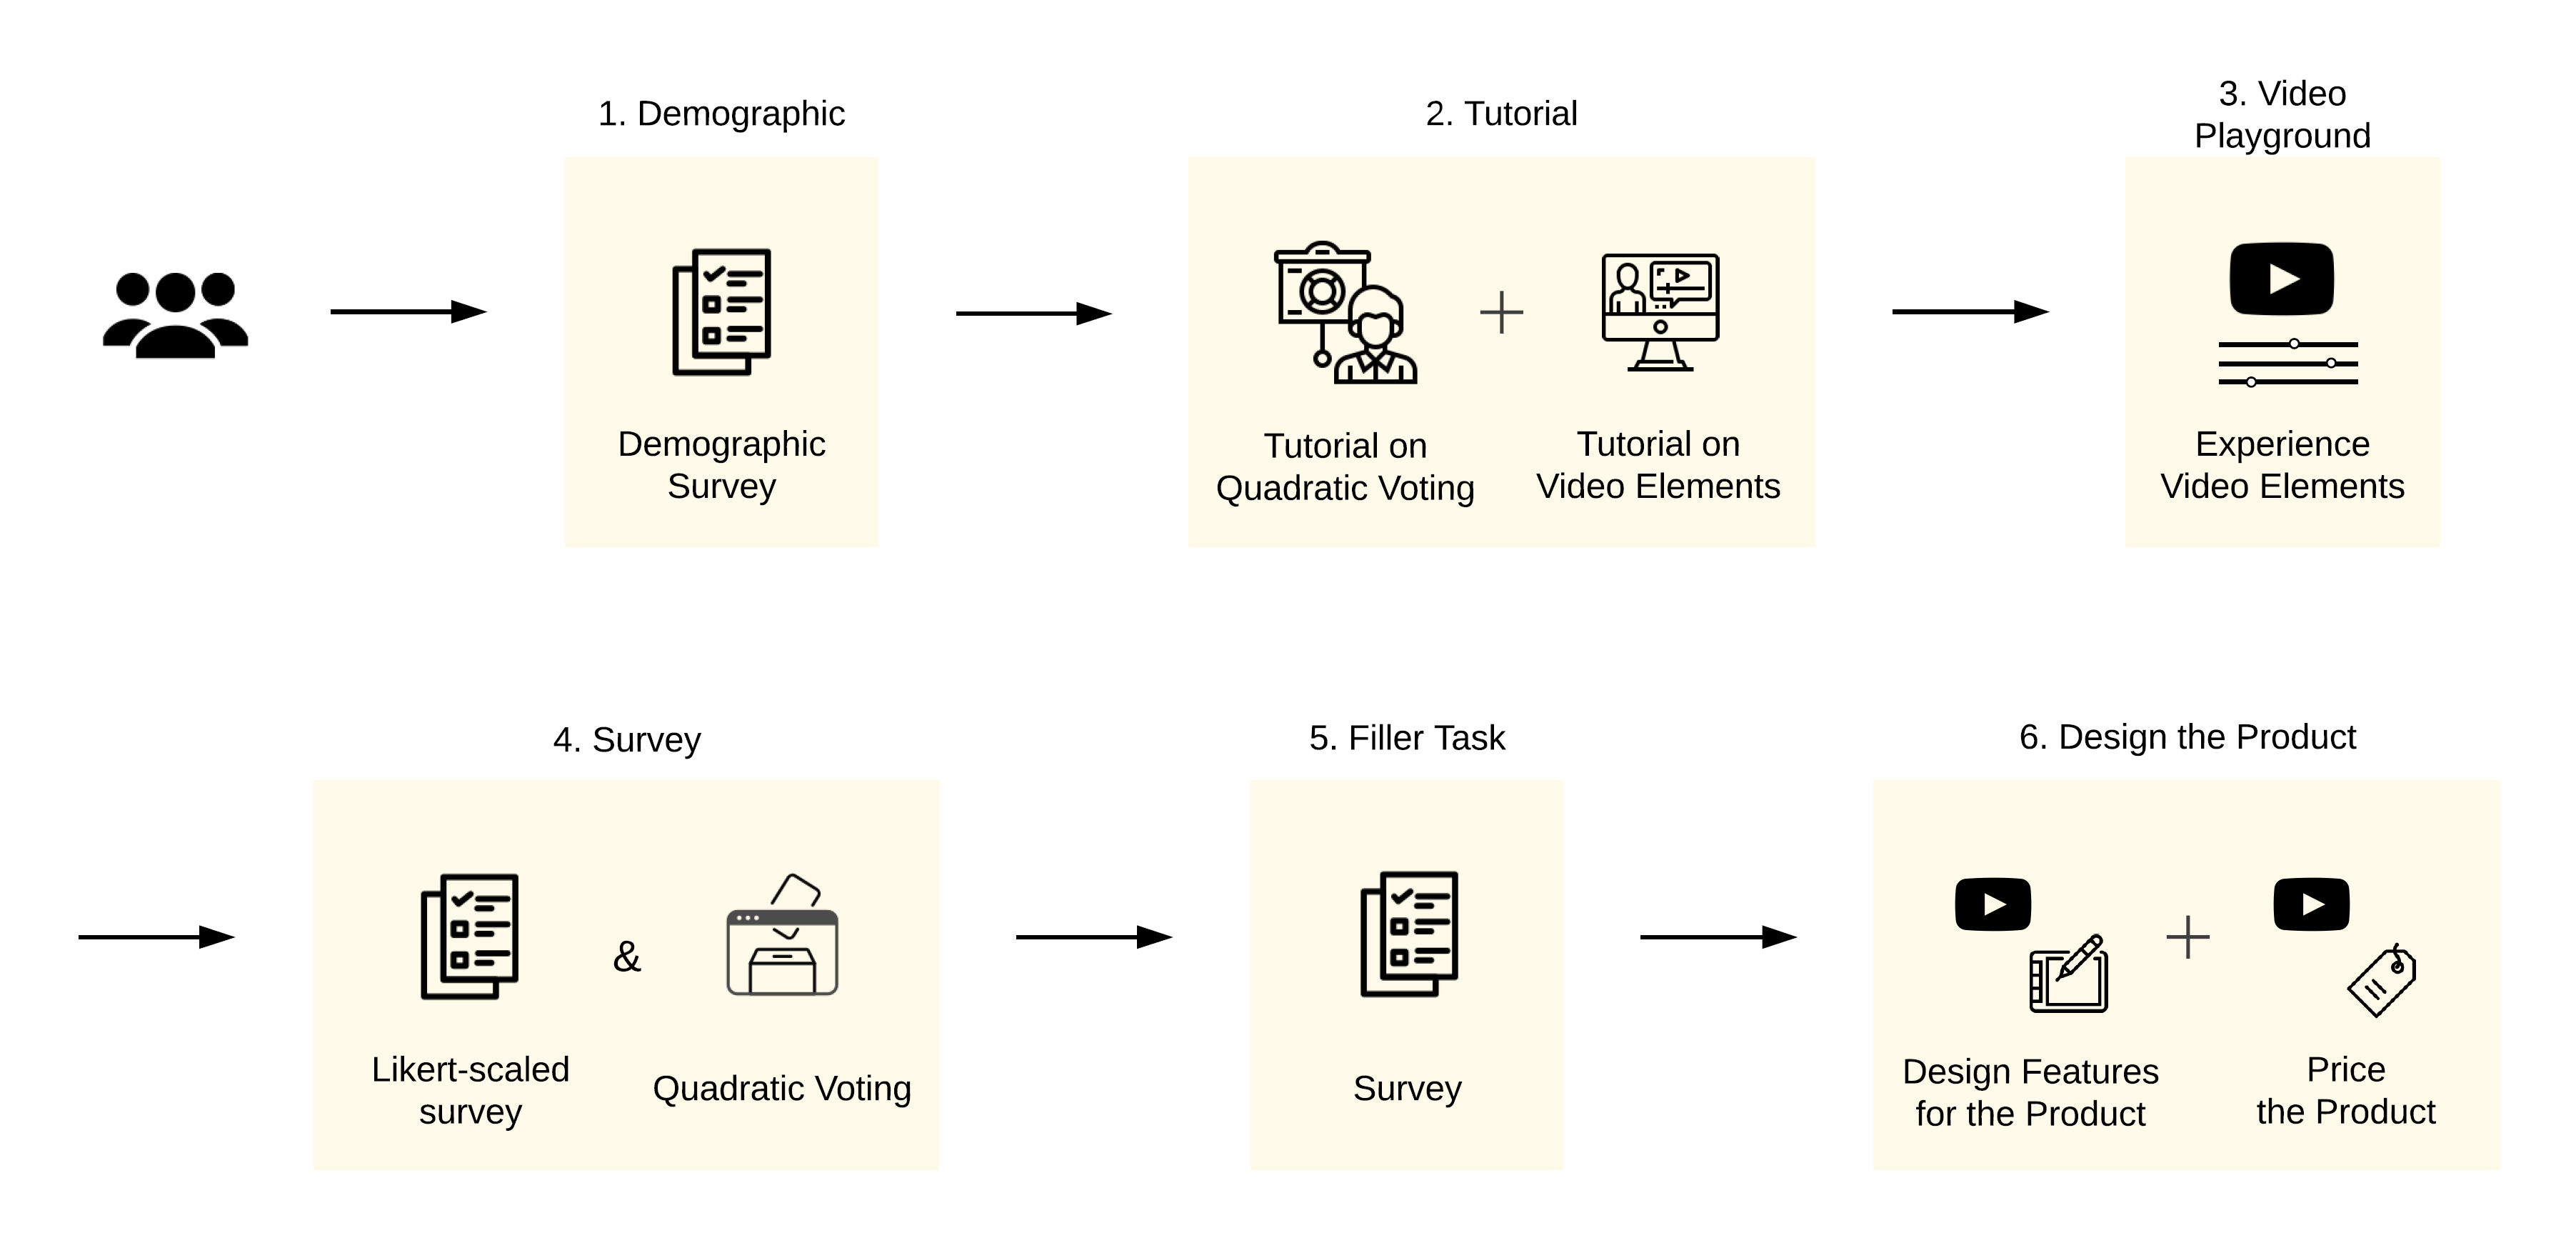
\includegraphics[width=\textwidth, keepaspectratio=true]{content/image/exp2_flow.png}
    \caption{
        Experiment one conducted between subjects. Participants were divieded into three groups. Participants that took the first path is the Likert Group, the center path is the QV group, and the bottom path is the buyback Group.
    }
    \label{fig:exp2_flow}
\end{figure}

\subsection{Experiment setup}
In this between-subject study, we recruit 180 participants through MTurk.
We equally distributed the participants into three groups, Likert group, QV group, buyback group listed in Figure \ref{fig:exp1_flow}, based on their demographic information.
Again, all three groups follow a similar experiment structure.
First, we ask participants to fill out the demographic survey identical to the first experiment.
All but the QV group will encounter the QV tutorial similar to the first experiment.
Then, each group visited a page that explained the five aforementioned video elements and completed a quiz.
This Quiz makes sure that the participants read through the content and understood the definition of the five video elements.

Participants will then have a chance to experience the video interface, to understand how different video elements impact a video (Fig \ref{fig:exp2_flow} ``Experiencing video elements'').
Participants were told that this research is conducted by a video streaming company primarily serving in-flight entertainment systems.
During flights, data bandwidth is limited and engineers of the company need to know what to prioritize to serve the customer.
We believe this scenario is easy to understand and can be easily applied to many real-life situations, such as a sudden drop in a mobile network, spotty WiFi connection, or unstable inflight internet.
We also believe that participants have experience degrade in at least one of the five video elements in the past, making this task easy to understand and relay.
To recreate such an environment, we built a video experience interface displayed in Figure \ref{fig:exp_2_video}.
This interface showcased a weather video with a set of controls at the bottom.
Participants can toggle any of these video elements, and see the immediate changes to the video on the top of the interface.
Participants can pause and play the video at any time.
As mentioned previously, we provided four levels of changes for each of the video elements. 
The four levels were selected based on previous studies and designed to be as linear to the user's perception as possible. 

For the Likert Group,
participants are also required to answer five sample questions
related to the video.
These questions are designed to assist participants
make sure they understood what the video is trying to convey.
Participants are also aware that 
there would be no penalties if they answered any of the questions incorrectly.
Once participants had spent enough time playing around with the video interface
and answered all five sample question, 
they are asked about the importance of the five video elements
using a Likert scale survey.
The five sample questions are essential to the experiment
because it primed all participants in the experiment to have the same goal of 
trying to understand the context of the video
and not just for pure entertainment purposes.

The QV group follows closely with the Likert Group.
Instead of presenting their attitude using a Likert scaled survey,
participants were asked to vote on how important they think
the different video elements were,
to help them comprehend the video content.
In this QV, we use 100 credits based on the optimal
results from the first experiment.
We use the same QV interface demonstrated in Figure \ref{fig:system_interface}.

The final group, the buyback group, completes a buyback task that mimics a rational customer's behavior:  buying essential tools to complete some given task.
Similar to the first experiment, we need a task to align the participant's attitudes with their behavior.
This task stems from many subscription-based services on the market, which requires customers to pay additional premiums for additional benefits.
%To the best of our knowledge, we are the first to design such a task, yet, it reflects many behaviors in real life.

During the first stage (Graph \ref{fig:exp2_flow} Buyback video elements), participants were given a video with sub-optimal quality that mimics worst-case scenarios if the internet bandwidth is limited. 
This is realized by setting the video interface controllers to level 0.
The video in the buyback stage is the same weather forecasting video demonstrated across all groups.
Participants can ``enhance'' each of these elements by``purchasing'' a level of that element. 
For instance, participants can buy two levels of audio quality and one level of video stability.
Each of these levels costs $2$ dollars. 
Participants were given a budget of \$30 to purchase some or all of the features back.
We call this action the ``buyback actions''.

To ensure the incentive-compatibility of the participants' buyback actions, we offered to pay the participants their own remaining amount from the \$30 budget through a lottery.
However, the eligibility to entire this lottery requires them to answer 80\% of five multiple-choice questions in the Quiz (Graph \ref{fig:exp2_flow} Quiz) correctly.
This Quiz comes with another weather forecast video, different from the previous one, using the set of controls the participants bought during the buyback.
This task set the goal for the participants, really considering the best use of their budget but understanding the content in the video.
The Quiz ensures that participants have correctly comprehended the video.

The five questions are factual questions such as, "What is the weather of Chicago?", "What is the highs and lows of San Diego," and "Which city was not shown in the video?". 
Participants were shown five example questions before the buyback task to assist their decision.
Participants can replay the video with their adjustments while answering the questions to ensure that participants do not require memorization.\par